%!TEX root=../../main.tex




\subsection{Galois speedup}
\label{sec:galois_speedup}
Analyzing the calculation time speedups for Galois, we can compare how or if the different algorithms benefit from increasing thread numbers.

\subsubsection{Single-source Shortest-path}
\begin{figure}
	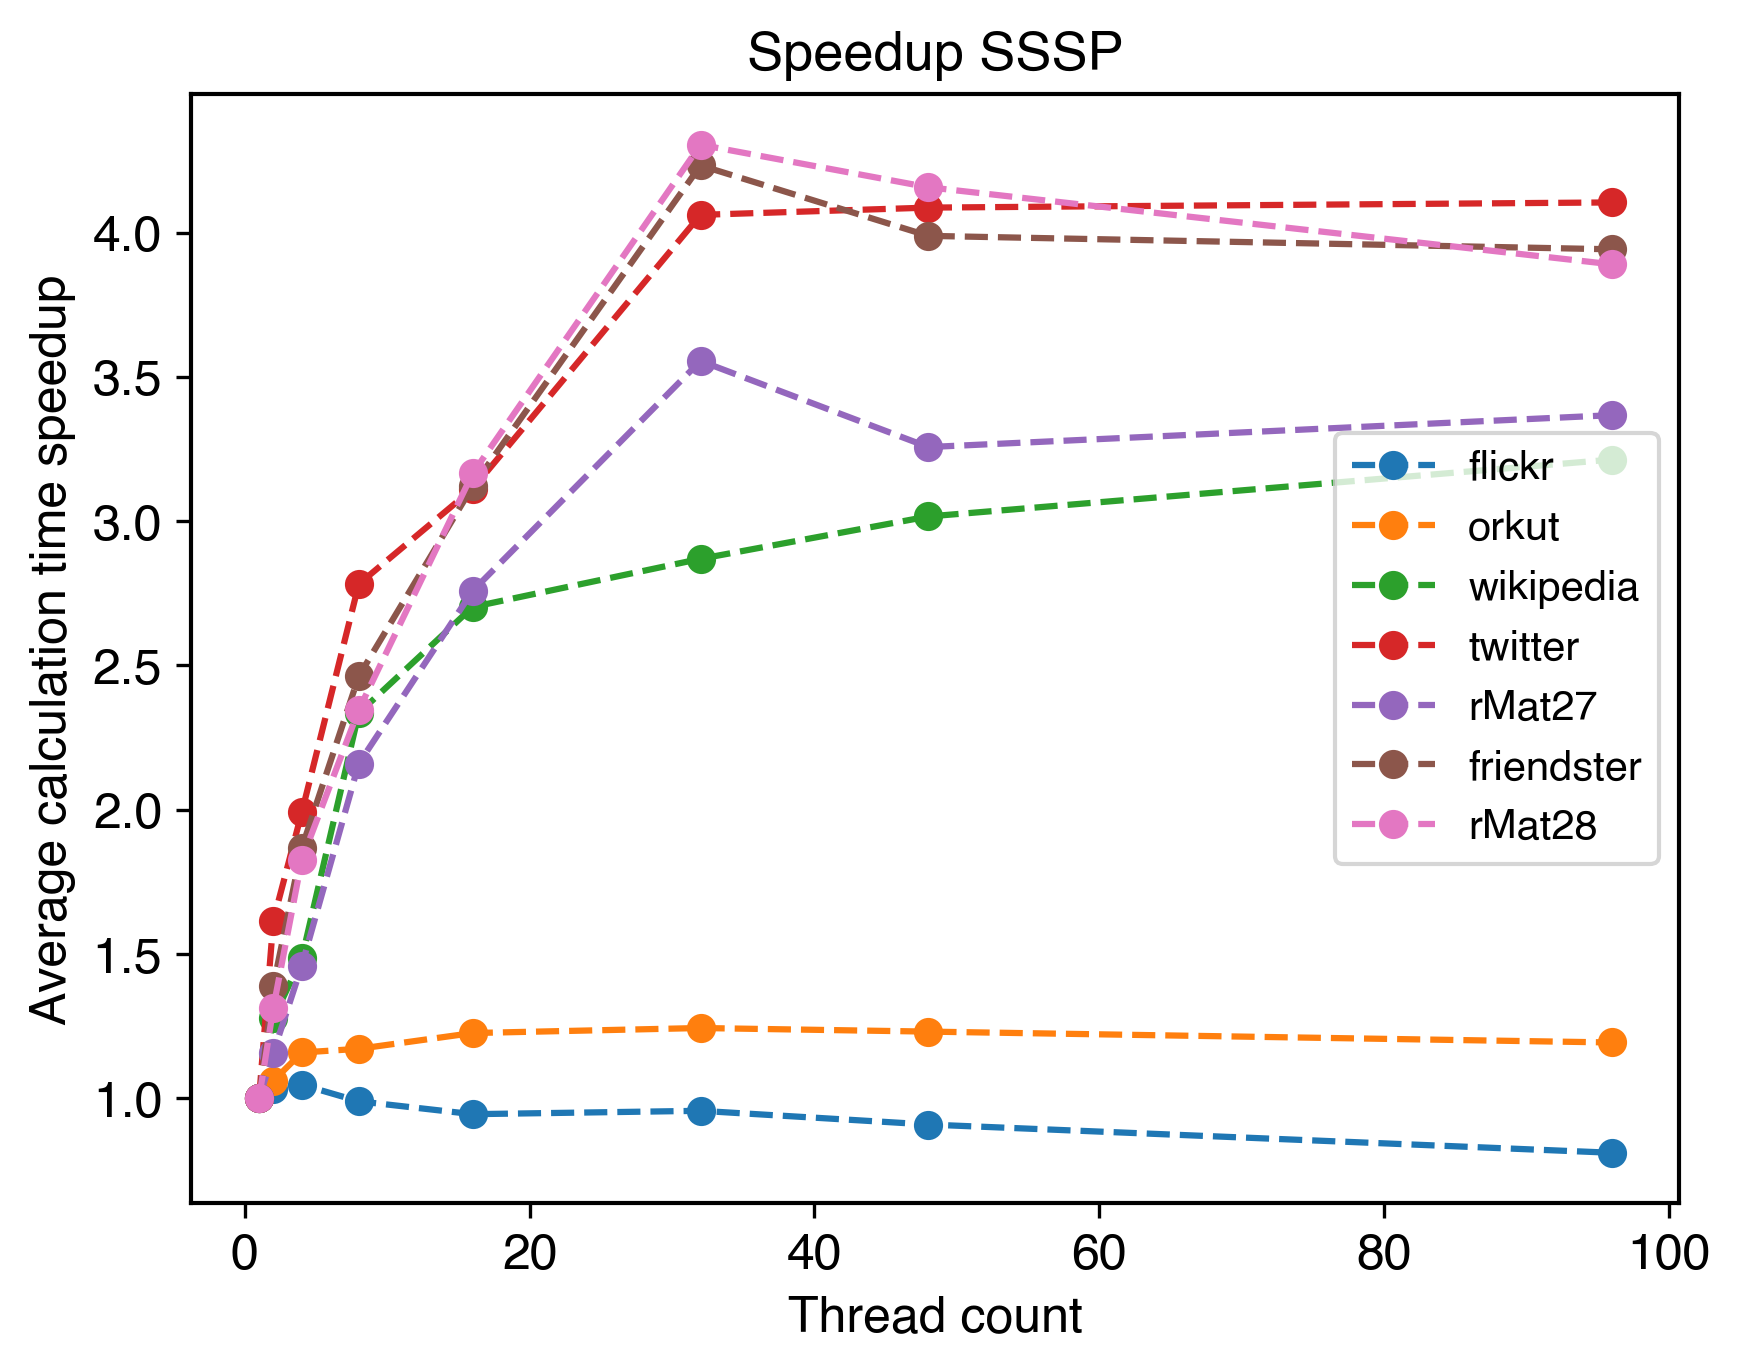
\includegraphics[width=\linewidth]{../../plots/singleNodeSSSPGaloisThreads.png}
	\caption{Calculation time speedup with increasing thread count for Galois Single-source Shortest-paths}
	\label{fig:galoisSpeedupSSSP}
\end{figure}
Starting with SSSP which is the algorithm that really is at an advantage when using many threads in \autoref{fig:galoisSpeedupSSSP}.

For all larger graphs, speedup is in most cases very close to optimal up to about 8 threads. 
Twitter has the best speedup, requiring only 38\%\ the calculation time with 2 threads compared to one, 25\%\ using 4 and 12.9\%\ using 8 threads.
Behaviour on friendster is similar with 52\%\ at 2 threads, 29\%\ at 4 and 16\%\ at 8 threads compared to one.

Anything above 32 threads however no longer helps decrease the computation time, in some cases even the opposite e.g. calculation on rMat28 is actually slower with 48 (13\% slower) or 96 threads (28\% slower) compared to 40 threads.

Small graphs like flickr or orkut, neither benefit from more threads nor is the performance held up by synchronization overhead. 



\subsubsection{Breadth-first search}
\begin{figure}
	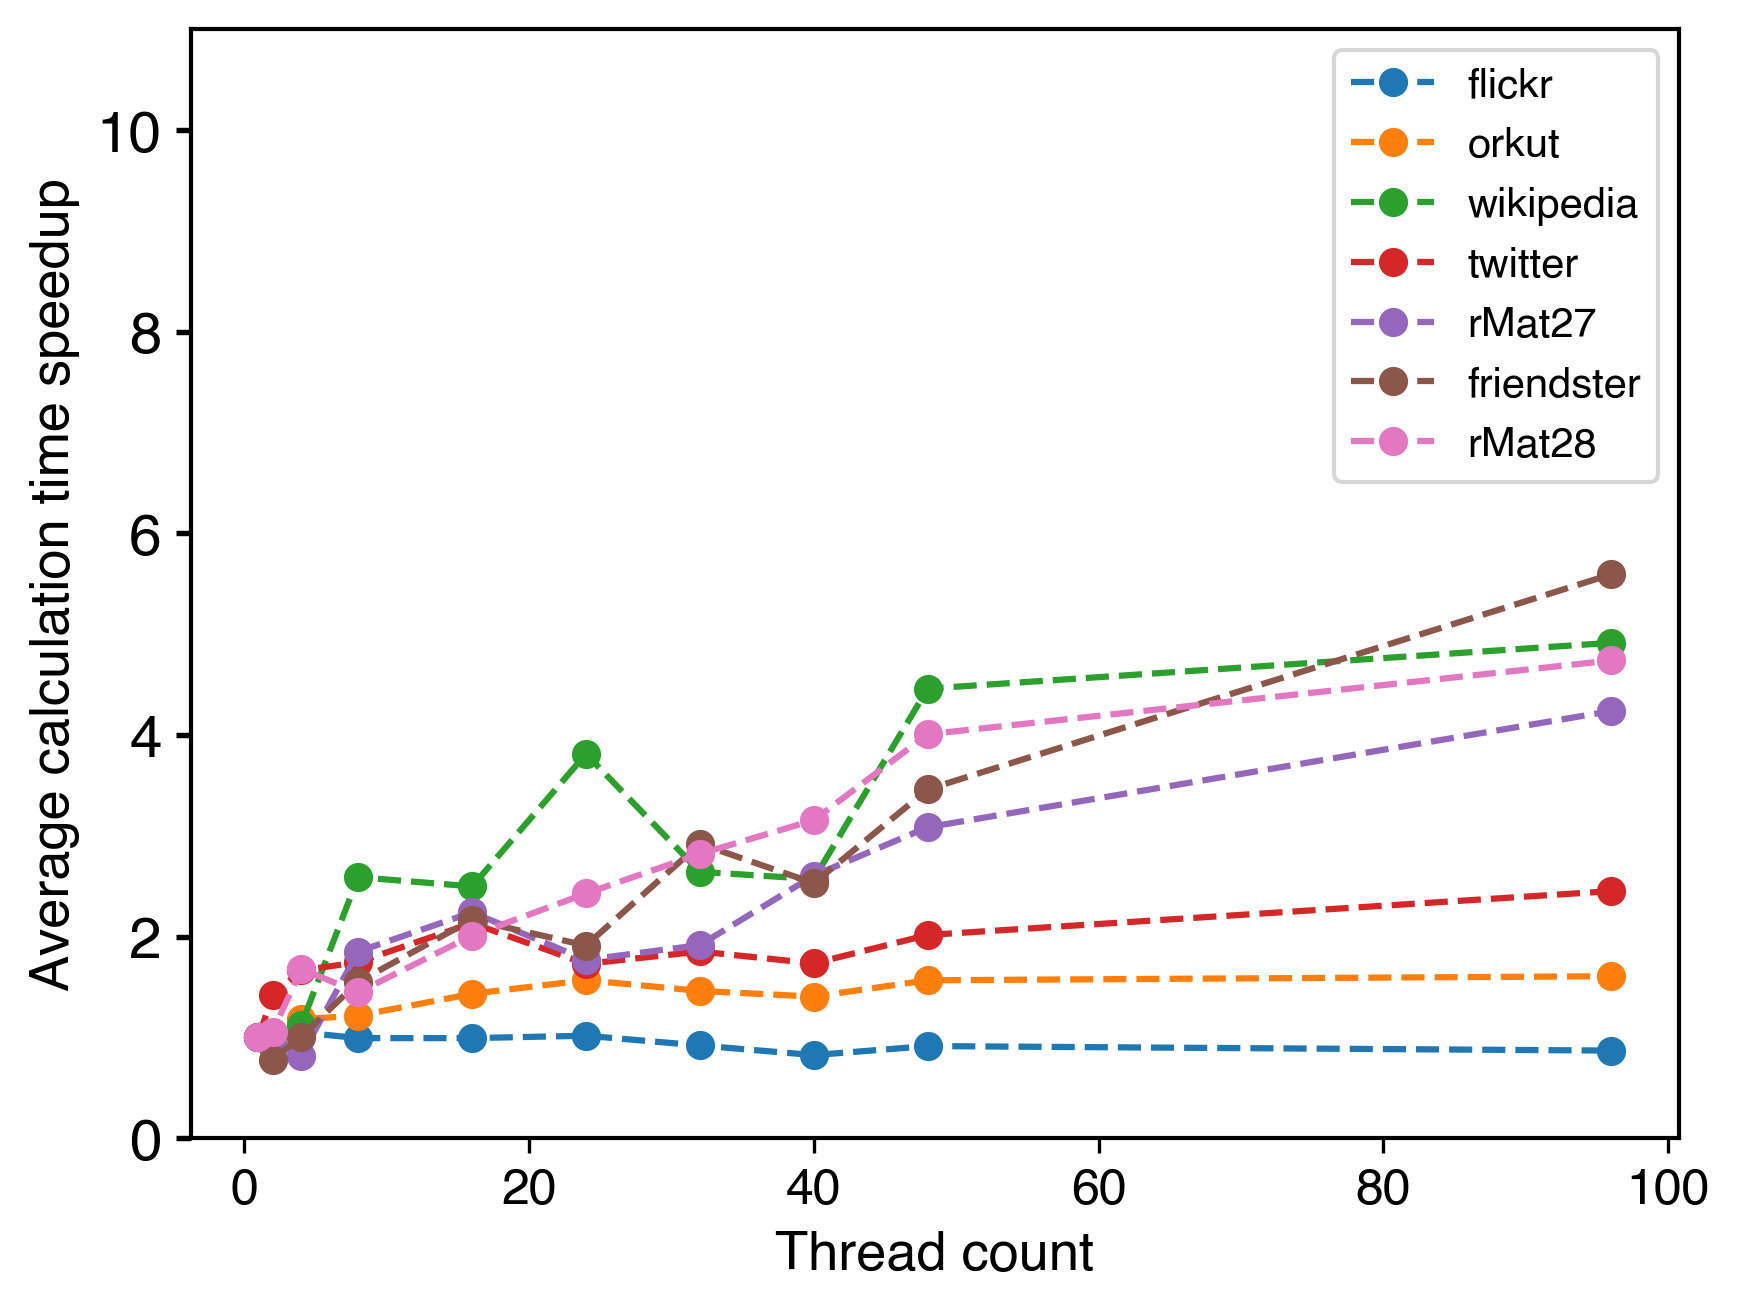
\includegraphics[width=\linewidth]{../../plots/singleNodeBFSGaloisThreads.png}
	\caption{Calculation time speedup with increasing thread count for Galois Breadth-first search}
	\label{fig:galoisSpeedupBFS}
\end{figure}

For our speedup results on BFS, \autoref{fig:galoisSpeedupBFS} shows the calculation time speedup of Galois' BFS.

Flickr is sped up by about 5\%\ with 4 threads, any more than that will actually decrease performance, making computation time up to 15\%\ (96 threads) longer.

On all graphs, the speedup never exceeds 6$\times$ even when using 96 thread.
The initial speedup when switching from one to two threads is actually smaller than one, thus decreasing performance, on 4 of 7 graphs. Only flickr, twitter and rMat28 can benefit slightly by a speedup of 2\%, 41\%\ and 5\%\ respectively.

When comparing four threads to one, BFS on all but two graphs can be sped up by anywhere from 5\%\ (flickr) to 68\% (rMat28). The speedup is thus only possible to a very small degree.
For the other two graphs, computation on friendster with 8 threads is just as fast as one thread and computation on rMat27 is actually 19\% slower.








\subsubsection{PageRank}
\begin{figure}
	\begin{subfigure}{\columnwidth}
		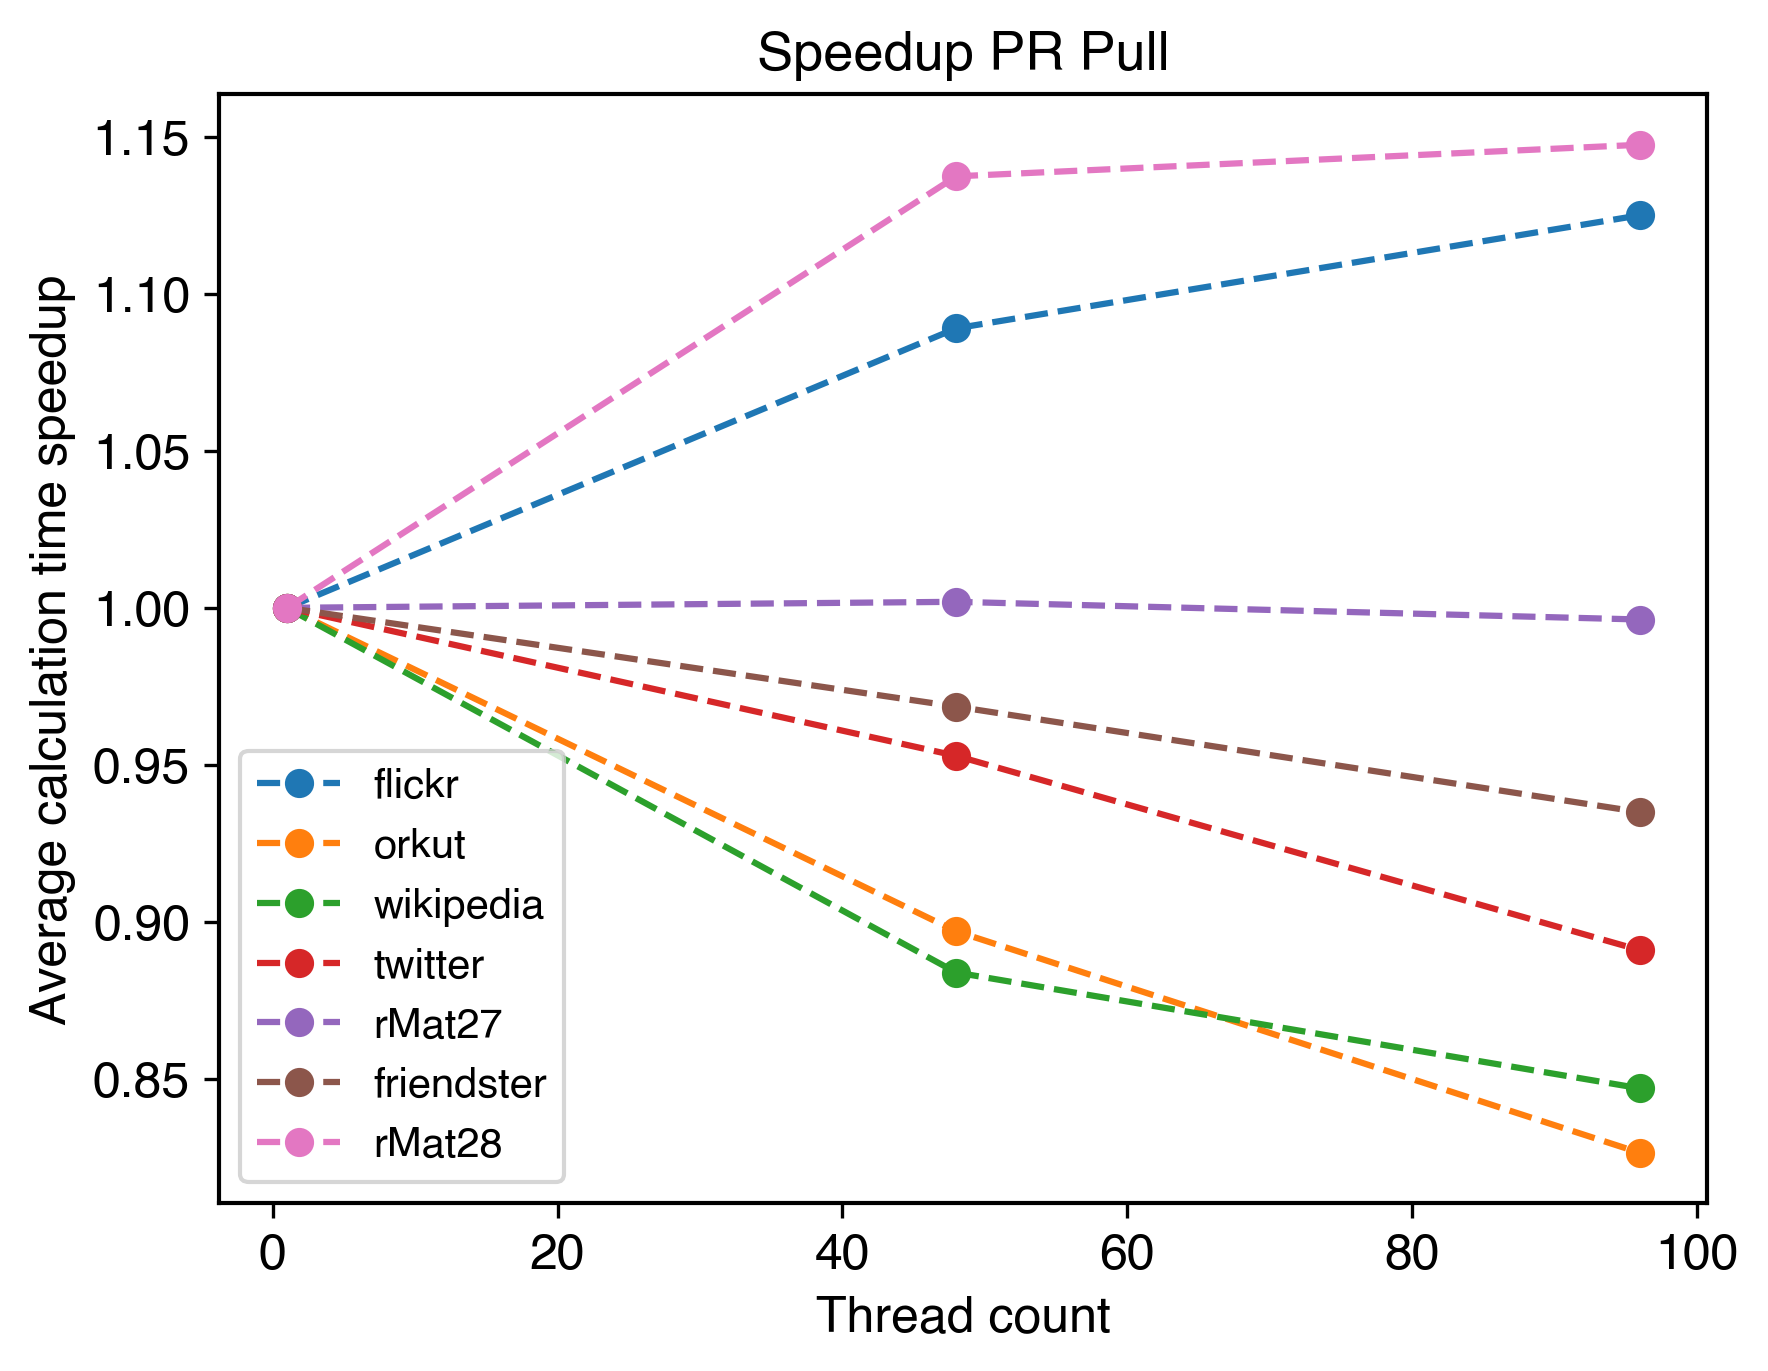
\includegraphics[width=\columnwidth]{../../plots/singleNodePRPullGaloisThreads.png}
		\caption{PageRank Pull}
		\label{fig:galoisSpeedupPRPull}
	\end{subfigure}
	\begin{subfigure}{\columnwidth}
		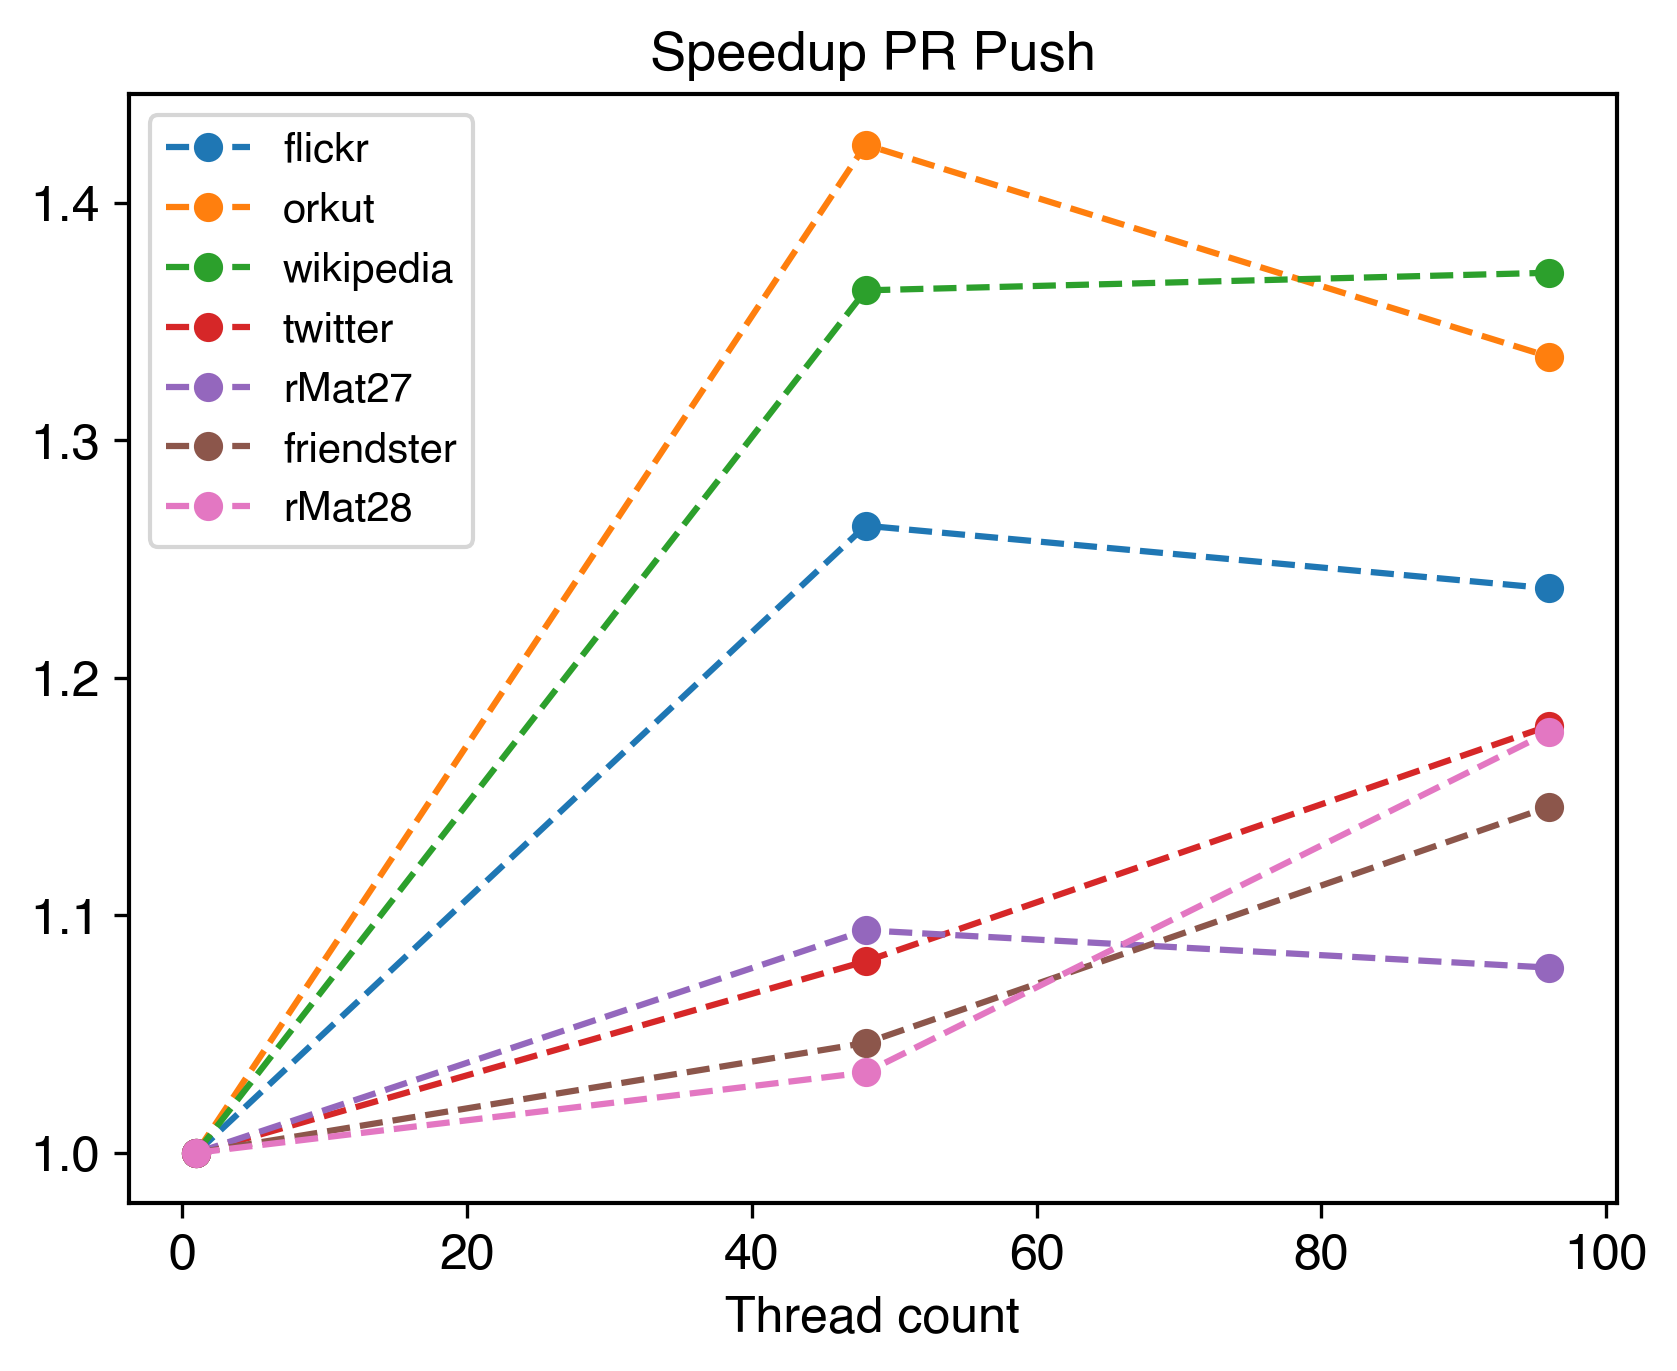
\includegraphics[width=\columnwidth]{../../plots/singleNodePRPushGaloisThreads.png}
		\caption{PageRank Push}
		\label{fig:galoisSpeedupPRPush}
	\end{subfigure}
	\caption{Calculation time speedup with increasing thread count for Galois PageRank Push and Pull algorithms.}
\end{figure}

